\section{Architecture}
\label{sec:archi}

Calcite contains many of the pieces that comprise a typical database management system. However, it omits some key components, \eg storage of data, algorithms to process data, and a repository for storing metadata. This decision is intentional: this makes Calcite an excellent choice for mediating between applications having one or more data storage locations and using multiple data processing engines. It is also a perfect foundation for building your own data processing system.

\begin{figure}[t]
\centering
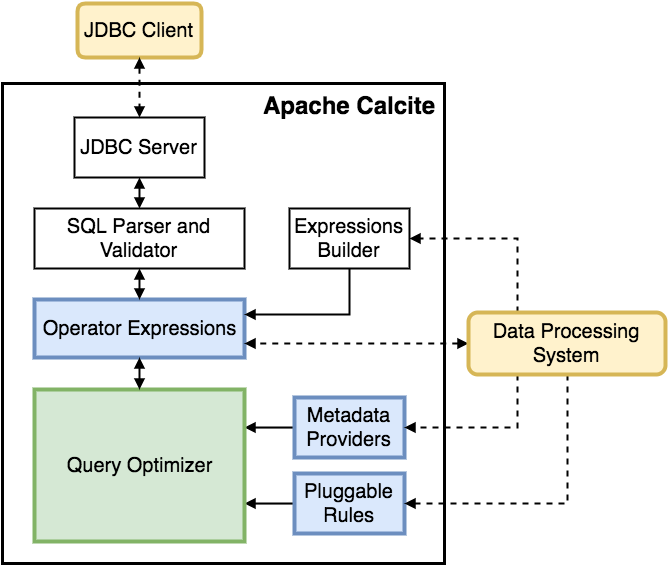
\includegraphics[width=0.94\columnwidth]{figures/architecture.png}
\vspacebfigure\caption{Apache Calcite architecture and interaction.\label{fig:arch}\JCR{Could we include the adapters in the figure?}}\vspaceafigure
\end{figure}

Figure~\ref{fig:arch} outlines the main components of Calcite's architecture. In the Figure, the dashed lines represent possible external interactions with the framework.

First of all, Calcite contains a query parser and validator that can translate a SQL query to a tree of relational operators. As we mentioned earlier, Calcite does not contain a \textit{storage layer}. Hence, it provides a mechanism to define table schemas and views using JSON files, so it can be used as a stand-alone system.

The tree of relational operators is the internal representation on which Calcite's optimizer works. The optimization engine consists mainly of three components which guide the process: rules, metadata providers, and planner engines. We talk about these components in more detail in Section~\ref{subsec:optimizer}.

Once the query has been optimized, Calcite can translate the relational expression back to SQL. Note that this allows Calcite to work as a stand-alone system on top of any data application with a SQL interface.

However, Calcite architecture is not only tailored towards this fashion of interacting with the framework. In fact, it is far more common that data processing systems choose to use their own parser for their own query language. In that case, Calcite also allows to easily build the operator tree directly instantiating the relational operators. Alternately, one can use the built-in \textit{relational expressions builder} interface. For instance, assume that we want to express the following SQL query using the expressions builder:

\begin{lstlisting}[language=SQL]
SELECT deptno, count(*) AS c, sum(sal) AS s
FROM emp
GROUP BY deptno;
\end{lstlisting}

The equivalent expression looks as follows:

\begin{lstlisting}[language=Java]
final RelNode node = builder
  .scan("EMP")
  .aggregate(builder.groupKey("DEPTNO"),
      builder.count(false, "C"),
      builder.sum(false, "S", builder.field("SAL")))
  .build();
\end{lstlisting}

Observe that the interface exposes the main constructs for building relational expressions. After the optimization phase is finished, the application can retrieve the optimized relational expression.

\subsection{Data model and type system}
\label{subsec:dm-ts}
Calcite's data model consists of three main entities.

\begin{itemize}
  \item \textbf{Schema} - A schema groups tables, streams, views and materialisations into one logical entity. A schema adapter~\ref{subsec:adapters} can be used to expose particular kind of data (e.g. Cassandra keyspace) as tables within a schema to Calcite.
  \item \textbf{Table} - A table is a typed collection of records defined by a set of named, strongly typed columns. Records in a table have no defined ordering.
  \item \textbf{Stream} - A stream is a possibly indefinite sequence of temporally-defined typed records. Each record in a stream should contain at least one monotonic or quasi-monotonic column that defines the order of records temporarily.
\end{itemize}

\MP{Please feel free to edit above. I am still not sure what we should mention about type system.}


\subsection{Relational expressions}
\label{subsec:relexprs}

Relational algebra~\cite{DBLP:journals/cacm/Codd70} lies at the core of Calcite. In addition to the operators that can be used to express the most common data manipulation operations, such as \textit{filter}, \textit{project}, \textit{join} \etc , Calcite includes additional operators that meet different purposes, \eg being able to concisely represent complex operations, or recognize optimization opportunities more efficiently.

For instance, it has become common for OLAP, decision making, and streaming applications to use window definitions to express complex analytic functions such as moving average of a quantity over a time period or number or rows.  Thus, Calcite introduces a \textit{window} operator that encapsulates the window definition, \ie upper and lower bound, partitioning \etc, and the aggregate functions to execute on each window.

Nevertheless, it is recommended that users combine existing operators wherever possible, rather than defining new ones. The core relational algebra is expressive, and adding a new operator requires adding a planner rule for each combination of the new operator with existing operators.

%%
\myparagraph{Traits.} Calcite does not use different entities to represent logical and physical operators. Instead, it describes the physical properties associated with an operator using \textit{traits}. These traits help the optimizer evaluate the cost of different alternative plans. It is important to note that if an operator property is considered a trait, changing its value does not change the logical expression being evaluated, \ie the rows produced by the given operator will still be the same.

During optimization, Calcite will try to enforce certain traits on relational expressions, \eg the sort order of certain columns. Relational operators can implement a \textit{converter} interface that indicates how to convert the physical attribute of the expression from one value to another.

Calcite includes common traits that describe the physical properties of the data produced by a relational expression, such as \textit{ordering}, \textit{grouping}, and \textit{partitioning}. Similar to~\cite{DBLP:conf/icde/ZhouLC10}, the optimizer can reason about these properties and exploit them to find plans that avoid unnecessary operations.

In addition to these properties, one of the main features of Calcite is the \textit{calling convention} trait. Essentially, the trait represents the data processing system on which the expression will be be executed. Including the calling convention as a trait allows Calcite to meet its goal of optimizing transparently queries whose execution might span over different engines \ie the convention will be treated as any other physical property.

\todo{Add figure}For example, consider joining a \textit{Products} table held in MySQL to an \textit{Orders} table held in Splunk. Initially, the scan of \textit{Orders} takes place in \textit{splunk} convention and the scan of \textit{Products} is in \textit{jdbc-mysql} convention (the tables have to be scanned inside their respective engines), and the join is in logical convention (meaning that no implementation has been chosen). One possible implementation is to use Apache Spark as an external engine: the join is converted to \textit{spark} convention, and its inputs are converters from \textit{jdbc-mysql} and \textit{splunk} to \textit{spark} convention. But there is a more efficient implementation: exploiting the fact that Splunk can perform lookups into MySQL via ODBC, a planner rule pushes the join through the \textit{splunk}-to-\textit{spark} converter, and the join is now in \textit{splunk} convention, running inside the Splunk engine.



\subsection{Query optimizer}
\label{subsec:optimizer}

The query optimizer is the main component in the framework. Calcite optimizes queries by repeatedly applying planner rules to a relational expression. A cost model guides the process, and the planner engine tries to generate an alternative expression that has the same semantics as the original but a lower cost.

Every component in the optimizer is extensible. One can add his own relational operators, rewriting rules, cost model, statistics, and even planner engine.

%%
\myparagraph{Rewriting rules.} Calcite includes a set of planner rules to transform expression trees. In particular, a rules matches a given pattern in the tree and executes a transformation that preserves semantics of that expression. At the moment of this writing, Calcite rules account to more than 75. However, it is rather common that data processing systems that rely for optimization on Calcite include their own rules, \eg\ to explore rewritings especially beneficial in that system.

\todo{Add figure with example of complex rule}

%%
\myparagraph{Metadata providers.} 

%%
\myparagraph{Planner engines.} 

%%
\myparagraph{Materialized views}



\subsection{Schema adapters}
\label{subsec:adapters}

\JCR{Before getting into detail about the adapters and how to implement them, it would help the reader to mention shortly what an adapter is; another line about them might be added to the beginning of the Section 2}

As discussed in Section~\ref{subsec:relexprs}, Calcite uses a physical trait to identify relational algebra operators which correspond to a specific database backend.
These physical operators implement the access paths for the underlying tables in each adapter.
When a query is parsed and converted to a relational algebra expression, an operator is created for each table representing a scan of the data on that table.
This represents the minimal interface that an adapter must implement.
If an adapter implements the table scan operator, the Calcite optimizer is then able to use client side operators such as sorting, filtering, and joins to execute arbitrary SQL queries against these tables.

To implement a table scan, a table exposed by an adapter must first be able convert itself to a relational algebra node.
This node contains the necessary information the adapter will require to issue he scan to the adapter's backend database.
The node inherits calling convention of the adapter.
To extend the functionality provided by adapters, Calcite defines an \emph{enumerable} calling convention.
Relational algebra nodes with the enumerable calling convention simply operate over tuples which can accessed via an iterator interface.
This allows Calcite to implement operators which may not be available in each adapter's backend.
For example, the \texttt{EnmerableJoin} operator implements joins by collecting rows from the iterators of its child nodes and joining on the desired attributes.

However, for queries which only touch a small subset of the data in a table, it is highly inefficient for Calcite to process queries by enumerating all tuples in a table.
Fortunately, the same rule-based optimizer can be used to implement adapter-specific rules for optimization.
For example, suppose a query involves filtering and sorting on a table.
An adapter which can perform filtering on the backend can implement a rule which matches a \texttt{LogicalFilter} and converts it to the adapter's calling convention.
This rules converts the \texttt{LogicalFilter} into another \texttt{Filter} instance.
This new \texttt{Filter} node has an associated cost that allows Calcite to optimize queries across adapters.
This rule will then store the necessary information so that when the request is made to the backend, the adapter will return results which have already been filtered.
Note that if the adapter does not support sorting, this sorting can still be performed within Calcite.

The use of adapters is a powerful abstraction that allows not only the optimization of queries for a specific backend, but also across multiple backends.
Calcite is able to answer queries which involve tables across multiple backends by pushing down all possible logic to each backend and then performing joins and aggregations on the resulting data.
Implementing an adapter can be as simple as providing a table scan operator or can extend to many advanced optimizations.
Any expression represented in the relational algebra for the query can be pushed down to adapters with optimizer rules.


\subsection{Streaming}
\label{subsec:streaming}

Some text.


